% Template for ICIP-2013 paper; to be used with:
%          spconf.sty  - ICASSP/ICIP LaTeX style file, and
%          IEEEbib.bst - IEEE bibliography style file.
% --------------------------------------------------------------------------
\documentclass{article}
\usepackage{spconf,amsmath,graphicx, subfigure}
\usepackage{hyperref}
% Example definitions.
% --------------------
\def\x{{\mathbf x}}
\def\L{{\cal L}}

% Title.
% ------
\title{Background Subtraction in Low-Quality Videos\\ with Subspace Estimation}
%
% Single address.
% ---------------
\name{Pooya Khorrami, Xingqian Xu, Mert Dikmen, Thomas S. Huang\thanks{This work was funded in part by the ONR grant N00014-12-1-0122. }}
\address{University of Illinois - Urbana Champaign \\ 
              %Department of Electrical and Computer Engineering\\
              Beckman Institute,  405 N. Mathews Avenue, Urbana IL, 61801, USA}
%
% For example:
% ------------
%\address{School\\
%	Department\\
%	Address}
%
% Two addresses (uncomment and modify for two-address case).
% ----------------------------------------------------------
%\twoauthors
%  {A. Author-one, B. Author-two\sthanks{Thanks to XYZ agency for funding.}}
%	{School A-B\\
%	Department A-B\\
%	Address A-B}
%  {C. Author-three, D. Author-four\sthanks{The fourth author performed the work
%	while at ...}}
%	{School C-D\\
%	Department C-D\\
%	Address C-D}
%
\begin{document}
%\ninept
%
\maketitle
%
\begin{abstract}
Gaussian Mixture Models (GMMs) are one of the most popular methods used for background subtraction in video processing today. However, noisy or low-quality videos make learning the underlying background model difficult and often lead to inaccurate foreground masks. To combat this, we propose representing the background using a low-rank subspace. In this paper, we demonstrate how subspace estimation techniques such as Robust Principal Component Analysis (Robust PCA) outperform GMMs on noisy traffic video sequences. We also introduce some modifications to the original Robust PCA algorithm and show how each of them improves the detection accuracy.
\end{abstract}
%
\begin{keywords}
Robust PCA, Subspace Estimation,  Subtraction Techniques, Image Analysis, Object Detection
\end{keywords}
%

\vspace{0.1in}

\section{Introduction}
%\label{sec:intro}
In the field of video surveillance, the user typically wishes to extract meaningful and salient information from a video sequence in a completely automatic fashion. In several instances, the video sequences are captured using stationary cameras leading to a relatively static scene layout. The absence of camera motion implies that the background of the video sequence exhibits very little variation while dynamic changes in the scene represent the objects of interest. In such cases, the most common approach is to perform background subtraction to separate said dynamic regions (i.e. foreground) from the background of each frame.

When performing background subtraction, some na\"ive methods include frame differencing and approximate median \cite{approxMed}. %Frame difference simply subtracts the current frame from the previous frame and the pixels where the difference exceeds a threshold are marked as foreground. The approximate median technique, on the other hand, models the background as the median of several past frames in the sequence. This median image is then subtracted from subsequent frames and pixels whose difference exceed a threshold are marked foreground. 
While these algorithms are simple to use and quite efficient, the most popular technique, by far, is adaptive  Gaussian Mixture Models (GMMs) \cite{FriedmanGMM, StaufferGMM}. These works posit that each pixel in the background image can be represented by a probability distribution formed by a mixture of Gaussians. If a pixel greatly deviates from its corresponding model, then the pixel is labeled foreground. While the number of Gaussians used at each pixel is usually fixed, there has been some work \cite{ZivGMM} that shows how the number of mixture components can be chosen adaptively.

Although background subtraction via GMMs enjoys widespread use in the computer vision community, it is not without drawbacks. As opposed to the frame differencing and approximate median techniques, GMMs possess several parameters that must be tuned individually. This implies that the algorithm is innately sensitive to different scene configurations and conditions. For example, GMMs are susceptible to non--Gaussian sensor noise found in low-quality videos, which leads to inaccurate foreground segmentations. Such sensitivities suggest a more robust algorithm is needed.

%Therefore it should be no surprise that GMMs tend to perform rather poorly on noisy videos where the foreground objects are not immediately distinguishable. 

When dealing with noisy video sequences, we advocate the use of low-rank subspaces for background subtraction.  %Given that each of the video sequences was obtained using a stationary camera, the high level of temporal redundancy between the frames suggests that the backgrounds lie on a low-dimensional subspace. 
In the case of stationary cameras, the high level of temporal redundancy between the frames suggests that the backgrounds lie on a low-dimensional subspace. Therefore, foreground activity can be thought of as sparse deviations from said subspace. In this paper, we will show empirically how subspace estimation techniques achieve superior performance to GMMs on noisy traffic video sequences. 

One of the most common subspace estimation techniques is Robust Principal Component Analysis (Robust PCA or RPCA) \cite{RPCA09} whose objective is to represent a data matrix (or video sequence) as the sum of a low-rank matrix (background) and a sparse matrix (foreground) via a convex optimization problem. Unfortunately, the algorithm is computationally expensive because it operates in batch on the entire sequence. To avoid this, one can use the Grassmannian Robust Adaptive Subspace Tracking Algorithm (GRASTA) by He et al. \cite{GRASTA12} which learns the low-rank subspace by subsampling the video frames and proceeds in an online fashion. While both methods have displayed great success, we will describe how performing Robust PCA on each of the video's color channels and using a reduced number of frames produces a new subspace estimation technique with more accurate results. 


The remainder of this paper is organized as follows. Section 2 will describe the improvements made to the batch Robust PCA algorithm. Section 3 will present our experimental setup and findings. Section 4 will describe our conclusions.


\begin{figure*}[htb]

\begin{minipage}[b]{0.3333\linewidth}
  \centering
  \centerline{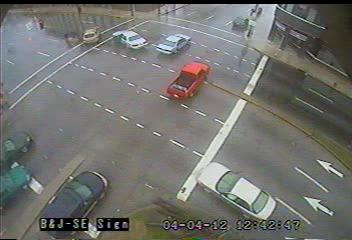
\includegraphics[width=5.55cm, height=3cm]{Imgs/Orig_0412041242.jpg}}
%  \vspace{2.0cm}
  \centerline{(a) Original Image}\medskip
\end{minipage}
%
\begin{minipage}[b]{0.3333\linewidth}
  \centering
  \centerline{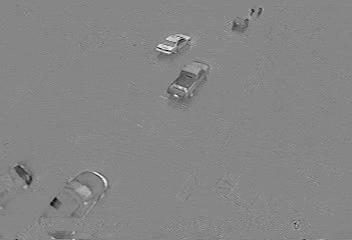
\includegraphics[width=5.55cm, height=3cm]{Imgs/SP_Intensity_0412041242}}
%  \vspace{1.5cm}
  \centerline{(b) Intensity Sparse Image}\medskip
\end{minipage}
\hfill
\begin{minipage}[b]{0.3333\linewidth}
  \centering
  \centerline{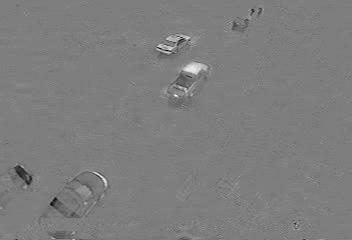
\includegraphics[width=5.55cm, height=3cm]{Imgs/SP_IMG_R_0412041242.jpg}}
%  \vspace{1.5cm}
  \centerline{(c) Red Channel Sparse Image}\medskip
\end{minipage}
%
\caption{Visual Comparison of Robust PCA on the Intensity Channel  and the Red Color Channel}
\label{fig:colorComp}
\medskip
%
\end{figure*}

\begin{figure*}[htb]

\begin{minipage}[b]{0.3333\linewidth}
  \centering
  \centerline{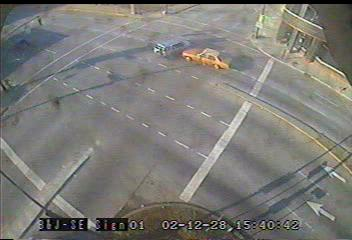
\includegraphics[width=5.55cm, height=3cm]{Imgs/Orig_1228021540.jpg}}
%  \vspace{2.0cm}
  \centerline{(a) Original Image}\medskip
\end{minipage}
%
\begin{minipage}[b]{0.3333\linewidth}
  \centering
  \centerline{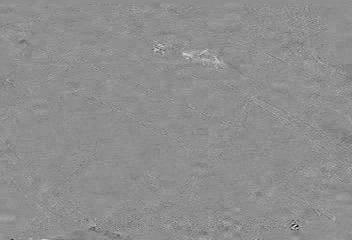
\includegraphics[width=5.55cm, height=3cm]{Imgs/SP_IMG_R_1228021540.jpg}}
%  \vspace{1.5cm}
  \centerline{(b) Robust PCA Sparse Image}\medskip
\end{minipage}
\hfill
\begin{minipage}[b]{0.3333\linewidth}
  \centering
  \centerline{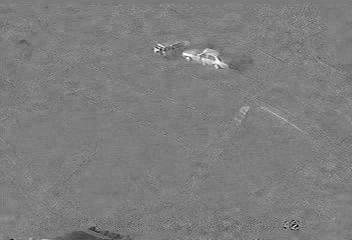
\includegraphics[width=5.55cm, height = 3cm]{Imgs/SP_IMG_Reduced_1228021540.jpg}}
%  \vspace{1.5cm}
  \centerline{(c) Reduced Robust PCA Sparse Image}\medskip
\end{minipage}
%
\caption{Reduced Frames Comparison}
\label{fig:reduceComp}
%
\end{figure*}

\section{Method Description}
%\label{sec:format}

When given a data matrix M, the goal of Robust PCA is to decompose it into a low-rank matrix L and a sparse matrix S. To do this, each of the video frames is vectorized and stacked as a column in the matrix M. Upon closer inspection, one will notice that the columns are highly correlated. %This is expected considering that the video was obtained using a stationary camera. 
Given that the background of a video lies on a low-dimensional subspace, we will see that the columns of L contain the background of each video frame and S contains the sparse deviations from that background, better known as foreground. Therefore, when doing background subtraction, one simply performs Robust PCA on the entire sequence and does further processing solely on the sparse error frames. While many works acknowledge the merit of using Robust PCA for background subtraction, very few have introduced modifications to improve foreground detection. 

In this section, we will present two particular changes we have made to improve Robust PCA's performance in background subtraction. They include: (1) individual modeling of the RGB color channels in order to distinguish objects based on color and (2) using a smaller number frames to reduce the time it takes for a foreground object to enter the background, better known as the foreground aperture problem.


\subsection{Robust PCA on Individual Color Channels}

Up until now, Robust PCA has only been performed on grayscale video sequences. However, color plays a crucial role in determining visually distinct or salient regions, especially when considering traffic sequences where cars are often identified by the color of their exterior. As such, we consider performing Robust PCA on all three of the color channels of a video sequence rather than just on the intensity channel. Now for each frame we have three sparse responses corresponding to each of the color channels. To ensure that an object detected with high confidence in one color channel is maintained in the final result, we take the maximum response across the three color channels.

Consider the images in Figure \ref{fig:colorComp}. After Robust PCA is performed on the intensity channel of the video sequence, we see in Figure \ref{fig:colorComp}b that several of the moving cars can be easily separated from the background just using their intensities. The red car, however, does not seem to stand out  from the background intensity. On the other hand, when considering the image in Figure \ref{fig:colorComp}c, we see that doing Robust PCA on the red color channel makes the red car very distinguishable. Given that we also take the maximum response across all the color channels, this high response will remain intact when extracting a foreground mask.

\subsection{Subsampling in time}

Now that we have a protocol in place to better detect colored objects, we turn our attention to detecting objects that have stopped moving. Ordinarily when a object has been stationary for a long period of time, the background subtraction algorithm considers it  to be a part of the background. Similarly with  Robust PCA, when an object is stationary it is no longer considered a sparse corruption. Rather, it is considered a basis element of the low-rank subspace and enters the frame's background. For instance, the cars shown in Figure \ref{fig:reduceComp}a have been stationary for some time, therefore they are no longer considered foreground and appear very faintly in the sparse component, shown in Figure \ref{fig:reduceComp}b.
 
In order to prevent this from happening, we reduce the number of frames used when computing Robust PCA by taking every Nth frame where N $\in \{ 10, 20, 30\}$. By reducing the number of frames in which the stationary object appears, we are making the object look like a sparse corruption and therefore less likely to enter the low-rank subspace modeling the background for the duration of the sampling period. The appearance of the two stationary cars in Figure \ref{fig:reduceComp}c verifies our hypothesis. The reader may have noticed that by using a reduced number of frames in Robust PCA, the remaining frames will not have their own low-rank and sparse components. This is not a problem given that the scene was captured using a stationary camera. For each frame, we can simply take the nearest background image and subtract it to extract the sparse component.

%\vspace{-0.23in}
\subsection{Post--processing}

After obtaining the sparse component of each video frame, we notice that they possess a fair amount of speckled noise. A classical approach to de-noising an image is through shrinking the wavelet coefficients via a hard or soft threshold \cite{Donoho95}. We apply a hard threshold to the wavelet coefficients of each color channel's sparse image prior to taking the max in order to obtain a smoother response to be used during evaluation.


\begin{figure}[t]
\centering
\begin{minipage}[b]{0.48\linewidth}
  \centering
  \centerline{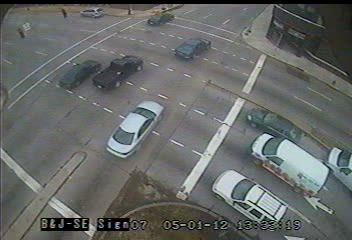
\includegraphics[width=4cm, height=2.8cm]{Imgs/0112051333.jpg}}
%  \vspace{2.0cm}
  \centerline{(a) Ground Truth Labels}\medskip
\end{minipage}
%\hfill
\begin{minipage}[b]{0.48\linewidth}
  \centering
  \centerline{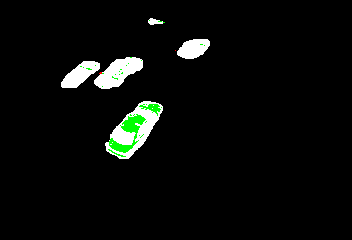
\includegraphics[width=4cm, height=2.8cm]{Imgs/0112051333_gmm_rwg.png}}
%  \vspace{1.5cm}
  \centerline{(b) GMM Result}\medskip
\end{minipage}

\begin{minipage}[b]{0.48\linewidth}
  \centering
  \centerline{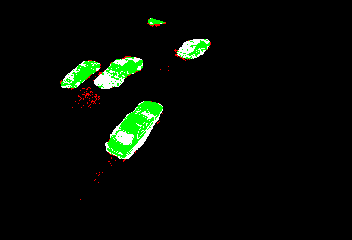
\includegraphics[width=4cm, height =2.8cm]{Imgs/0112051333_grasta_rwg.png}}
%  \vspace{1.5cm}
  \centerline{(c) GRASTA Result}\medskip
\end{minipage}
%\hfill
\begin{minipage}[b]{0.48\linewidth}
  \centering
  \centerline{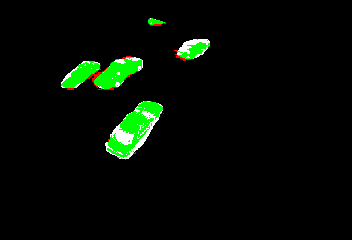
\includegraphics[width=4cm, height = 2.8cm]{Imgs/0112051333_rpca_rwg.png}}
%  \vspace{1.5cm}
  \centerline{(d) Our Result}\medskip
\end{minipage}

\caption{Method Comparison I - (White - Ground Truth, Red - False Positive, Green -  True Positive)}
\label{fig:methodComp1}
%
\end{figure}


\begin{figure}[t]
\centering
\begin{minipage}[b]{0.48\linewidth}
  \centering
  \centerline{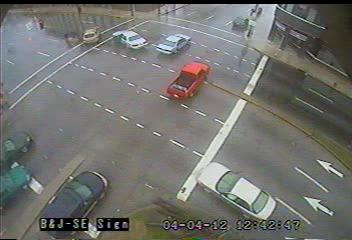
\includegraphics[width=4cm, height=2.8cm]{Imgs/0412041242.jpg}}
%  \vspace{2.0cm}
  \centerline{(a) Ground Truth Labels}\medskip
\end{minipage}
%\hfill
\begin{minipage}[b]{0.48\linewidth}
  \centering
  \centerline{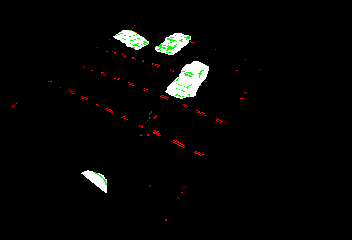
\includegraphics[width=4cm, height=2.8cm]{Imgs/0412041242_gmm_rwg.png}}
%  \vspace{1.5cm}
  \centerline{(b) GMM Result}\medskip
\end{minipage}

\begin{minipage}[b]{0.48\linewidth}
  \centering
  \centerline{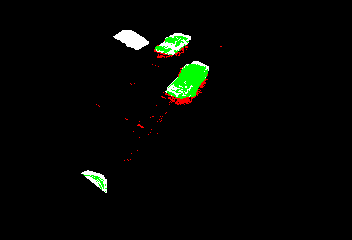
\includegraphics[width=4cm, height =2.8cm]{Imgs/0412041242_grasta_rwg.png}}
%  \vspace{1.5cm}
  \centerline{(c) GRASTA Result}\medskip
\end{minipage}
%\hfill
\begin{minipage}[b]{0.48\linewidth}
  \centering
  \centerline{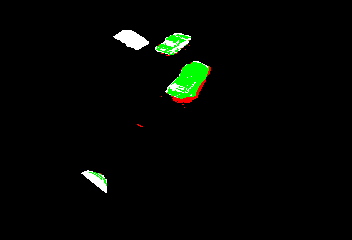
\includegraphics[width=4cm, height = 2.8cm]{Imgs/0412041242_rpca_rwg.png}}
%  \vspace{1.5cm}
  \centerline{(d) Our Result}\medskip
\end{minipage}

\caption{Method Comparison II - (White - Ground Truth, Red - False Positive, Green -  True Positive)}
\label{fig:methodComp2}
%
\end{figure}

\section{Experimental Results}
For evaluation, we use a dataset provided by Toyota Motor Corp. consisting of accidents and near accidents in a busy intersection in Louisville, KY area.  Parts of this dataset is available in the TRIMARC dataset\cite{toyota_dataset}.  The dataset contains video clips of 116 accidents and 235 near accidents,  ranging 10-30 seconds in duration.  The frames are of fairly low resolution (240$\mathbf{x}$320). In some of these videos, the camera sensor is defective resulting in washed out nighttime or off--color daytime images.  After pruning such cases, we manually marked ground truth labels for all foreground pixels in one frame for each of the 272 remaining videos.  The labeled frames are precisely seven seconds prior to end of each video, where the incident has either just occurred or is about to occur.  This makes sure that the intersection contains a fair amount of vehicles and provides some challenging cases where some vehicles became stationary after colliding.  In addition, the dataset, collected over the span of five years, contains many challenging environmental conditions such as wet or snowy roads, varying levels of day and nighttime illumination and significant amounts of CCD sensor noise. These annotations are  publicly available at \cite{datasetLink}. 


We test our hypothesis empirically on this dataset by comparing our results to a baseline GMM\cite{ZivGMM} algorithm.  The implementation is publicly available in OpenCV\cite{opencv_library}.  The parameters used for this particular GMM implementation were two Gaussian mixtures and 10 frames of history.  To get different operating points, we initialized the models with varying levels of foreground threshold corresponding to $\sigma \in \{0.5, 1, 2, 3, 4, 5\}$, and ran the background subtractor from the beginning of the video until the frame with the ground truth label.

\begin{figure}[htb]
\begin{minipage}[b]{\linewidth}
  \centering
  \centerline{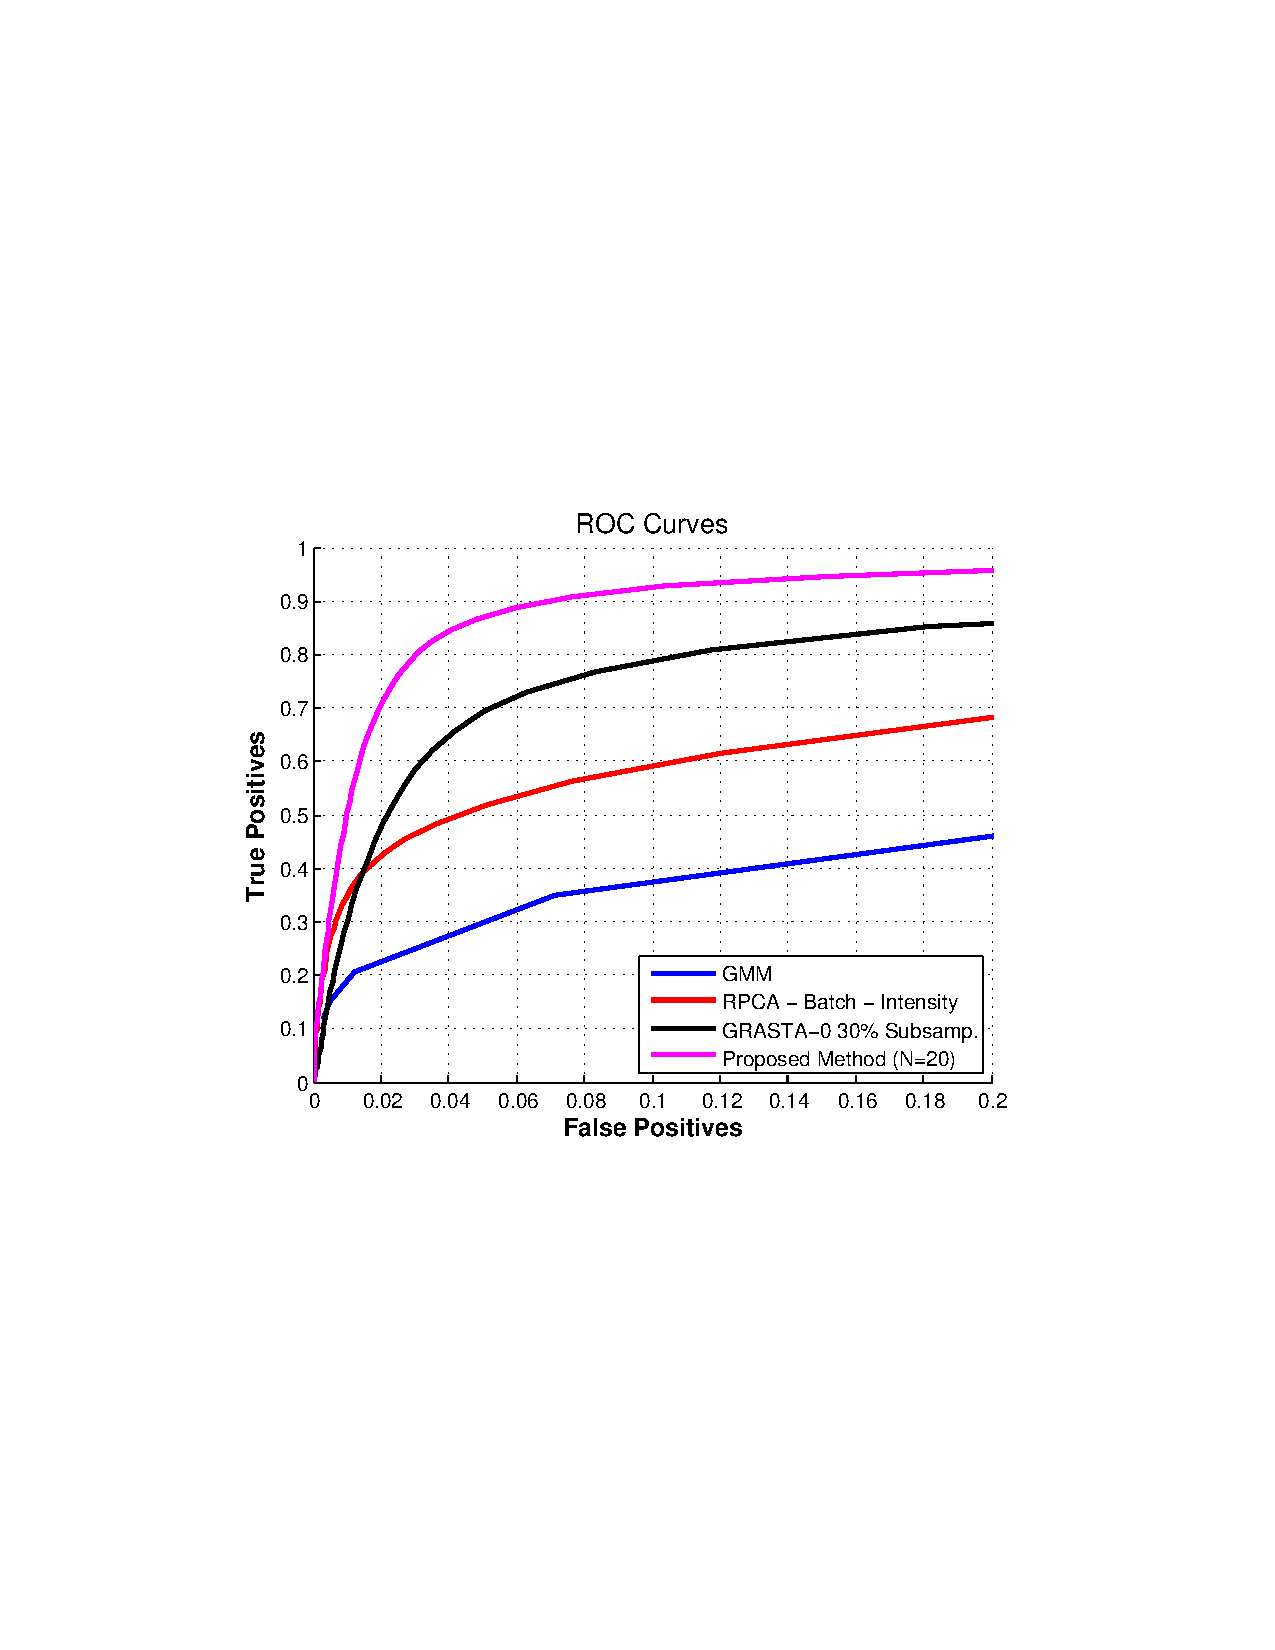
\includegraphics[trim = 35mm 87mm 30mm 92mm, clip,  width=9.25cm, height = 6.5cm]{Imgs/ROC_comp_curve_zoom.pdf}}
%  \vspace{1.5cm}
%  \centerline{(}\medskip
\end{minipage}

\caption{Algorithm Comparison}
\label{fig:roc}
\end{figure}


When computing Robust PCA, we used the Inexact Augmented Lagrangian method (IALM) \cite{alm} \cite{rpcaCode} with $\lambda = \frac{1}{\sqrt{MN}}$ where each frame is $M\times N $ pixels. For GRASTA, we used the code provided on the author's website \cite{grastaCode}. We trained the initial background model by taking 50 frames and subsampling 30$\%$ of the pixels while iterating 10 times. Then, during evaluation we applied the learned subspace and subsampled 20$\%$ of the pixels in the new frames. For our method, we performed Robust PCA on each of the color channels and took every 20th frame for training. Then for every testing frame, we used the background frame closest to it in time to extract the foreground. Since each video sequence was approximately 300 frames in length, taking every 20th frame corresponded to training on 15 frames in total. We took every 20th frame to ensure that both our method and GRASTA used the same number of frames during training since GRASTA subsampled 30$\%$ of the 50 training frames which is equal to 15 frames worth of pixels.

We quantify the performance of different approaches in terms of receiver operating characteristic curves (ROC).  We treat the foreground background labeling as a pixel--wise binary classification problem.  The true positive rate denotes the ratio of foreground pixels correctly detected by the particular algorithm versus the total number of foreground pixels in the ground truth set.  Conversely, the false positive ratio corresponds to the ratio of background pixels mistakenly picked up as foreground versus the total number of background pixels in the ground truth set.
%\label{sec:pagestyle}

The ROC curves in Figure \ref{fig:roc} show that the sparsity enforcing methods are better suited to handle adverse imaging conditions of the tested video shots.  One particular advantage is that GMMs are fairly slow to adapt to changes, while the subspace methods can adapt more rapidly to global changes while still being able to maintain the foreground objects for some time after they have become stationary. We also provide some qualitative results in Figures \ref{fig:methodComp1} and \ref{fig:methodComp2} to illustrate some of the advantages.  In Figure \ref{fig:methodComp1}, we can see that the some cars are assigned as background by the GMM algorithm, because the color separation between the background and the foreground does not make it above the threshold.  Whereas the majority of the foreground pixels are recovered by the subspace methods.  In Figure \ref{fig:methodComp2}, we see that some lane markings are picked up as foreground by the GMM method, possibly due to small camera motion causing misalignment of the background model.  However the subspace methods are able to capture such globally structural changes.

\begin{figure}[t]
\begin{minipage}[b]{\linewidth}
  \centering
  \centerline{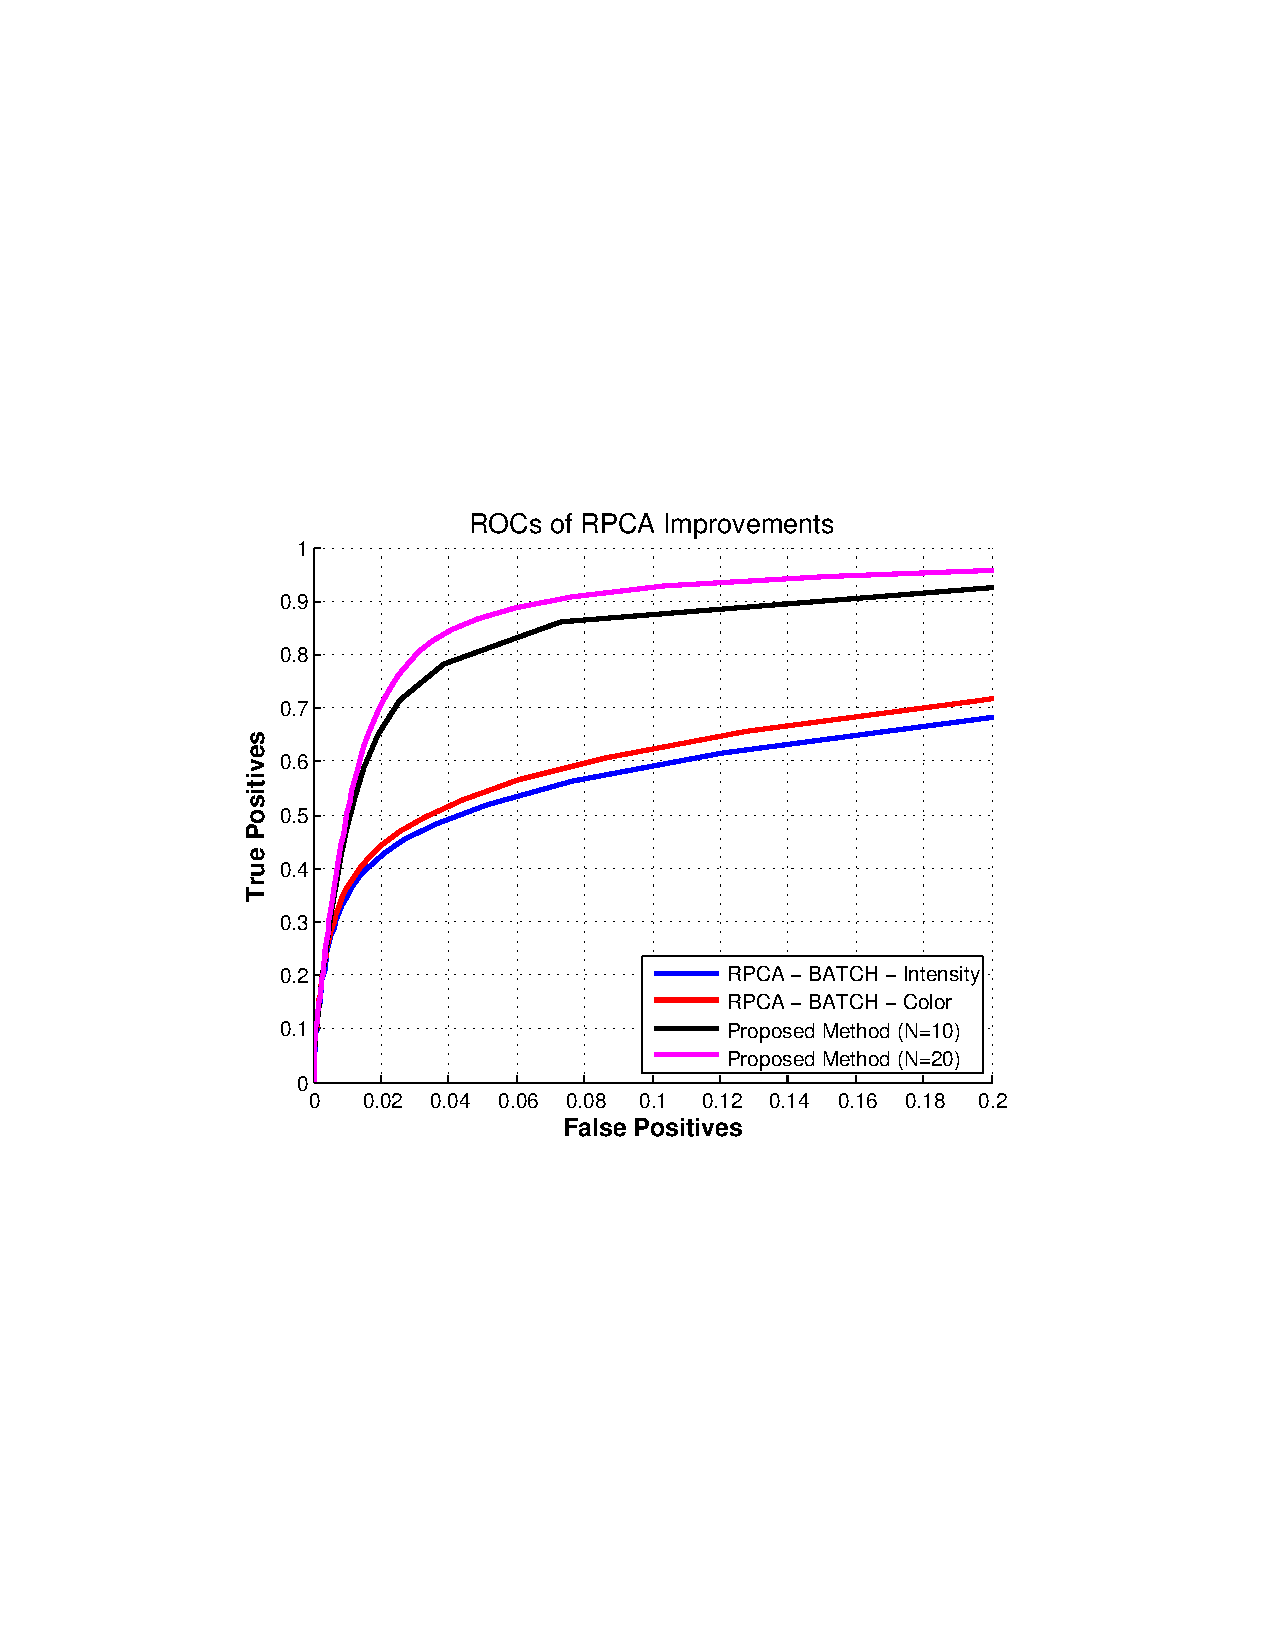
\includegraphics[trim = 35mm 87mm 30mm 92mm, clip, width=9.25cm, height =6.5cm]{Imgs/ROC_RPCA_IMP.pdf}}
%  \vspace{1.5cm}
%  \centerline{(}\medskip
\end{minipage}

\caption{Performance Gains due to RPCA Modifications}
\label{fig:roc2}
%\vspace{-0.15in}
\end{figure}


Figures \ref{fig:methodComp1}, \ref{fig:methodComp2} and \ref{fig:roc} also indicate how our algorithm outperforms all of the previously proposed methods by a fair margin, both quantitatively and qualitatively. In Figure \ref{fig:roc2}, we show how each of the modifications we proposed to the original Robust PCA algorithm leads to incremental improvements in the algorithm's performance. We see that incorporating color information yields a slight improvement over the original algorithm while using color in conjunction with a reduced number of frames produces a major improvement. Moreover, taking fewer and fewer frames when computing RPCA also leads to an increase in detection accuracy. This is expected given that stationary cars are now viewed more infrequently and will instead be classified as foreground.%The blue and red curves show the performance of batch Roust PCA when using intensity and color, respectively. The black and magenta curves show how using fewer and fewer frames when learning the subspace further improves the performance by reducing the effect of the foreground aperture problem. The black curve represents using every 10th frame (30 frames total) while the magenta curve represents using every 20th frame (15 frames total). 



\section{Conclusions}
We have demonstrated that under adverse imaging conditions, the limitations of commonly used Gaussian Mixture Models for background subtraction can be overcome by alternative robust methods that model the scene background as mixture of linear subspaces. We have also shown how our proposed modifications to Robust PCA led to marked gains in performance when compared to the original method as well as other popular subspace methods such as GRASTA.




%One important drawback of using subspace methods like RPCA is that the additional computational complexity brought on can be prohibitively expensive for real time processing under practical application conditions.  Thus we also evaluated the alternative GRASTA method, which has the ability to process fast on--line updates.  We have shown that, while some accuracy is sacrificed, the results obtained by GRASTA method is still largely favorable to GMM results.



%\label{sec:typestyle}



% References should be produced using the bibtex program from suitable
% BiBTeX files (here: strings, refs, manuals). The IEEEbib.bst bibliography
% style file from IEEE produces unsorted bibliography list.
% -------------------------------------------------------------------------
\bibliographystyle{IEEEbib}
\bibliography{strings,refs}

\end{document}
